\chapter{Git和GitHub简介}
在本章的最开始,我们先做一个本质的区分:
\begin{quotation}
    \textit{Git:一个用于用于版本控制的软件}

    \textit{Github:运营的网站,协作式源代码托管网站}
\end{quotation}

相信在阅读过程中,你能逐渐体会到两者的差异和联系。

\section{Git}
Git 是一个开源免费的分布式版本管理系统,由芬兰程序员 Linus Torvalds 开发。Git 的版本控制可以对代码、文档和日常工作所用到的文件进行方便的管理,而不用多次对源代码进行复制。还可以在多人合作的项目中可以记录所有的版本信息,同步不同来源的改动并在不同的地方备份整个项目。

\subsection{Git的基本概念}
本部分参考了\cite{git-cong}的内容。
\subsubsection{版本控制系统}
Git 是目前世界上最优秀的分布式版本控制系统。版本控制系统是能够随着时间的推进记录一系列文件的变化以便于你以后想要的退回到某个版本的系统。版本控制系统分为三大类:本地版本控制系统,集中式版本控制系统和分布式版本控制系统。

本地版本控制(Local Version Control Systems)是将文件的各个版本以一定的数据格式存储在本地的磁盘(有的VCS 是保存文件的变化补丁,即在文件内容变化时计算出差量保存起来),如图\ref{lo-me-con}左所示。这种方式在一定程度上解决了手动复制粘贴的问题,但无法解决多人协作的问题。

集中式版本控制(Centralized Version Control Systems)相比本地版本控制没有什么本质的变化,只是多了个一个中央服务器,各个版本的数据库存储在中央服务器,管理员可以控制开发人员的权限,而开发人员也可以从中央服务器拉取数据,如图\ref{lo-me-con}右所示。集中式版本控制虽然解决了团队协作问题,但缺点也很明显:所有数据存储在中央服务器,服务器一旦宕机或者磁盘损坏,会造成不可估量的损失。

\begin{figure}[ht]
    \centering
    \begin{minipage}[c]{0.45\textwidth}
        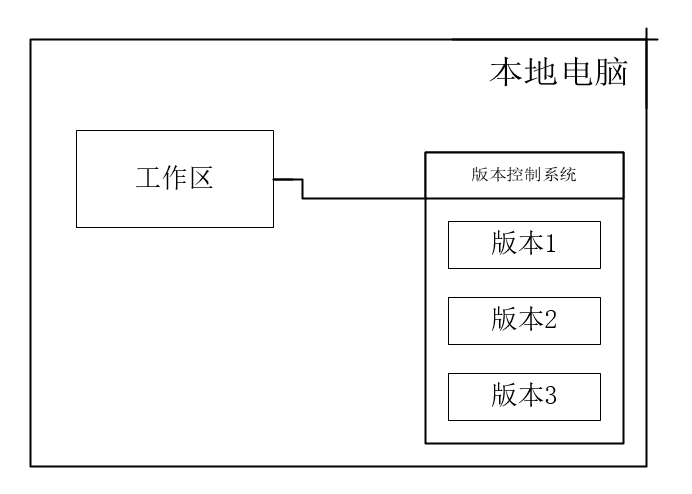
\includegraphics[width=\textwidth]{image/git/local-ver-control.png}
    \end{minipage}
    \begin{minipage}[c]{0.45\textwidth}
        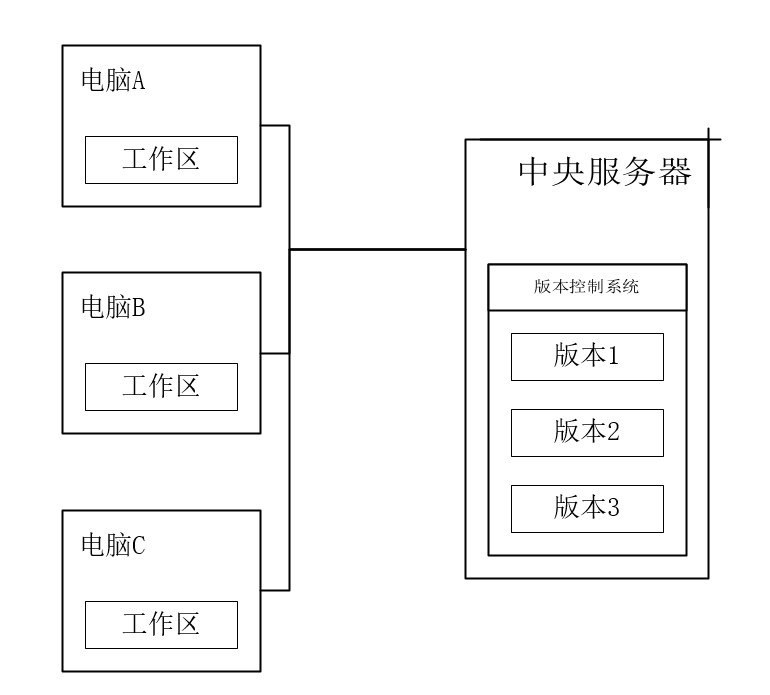
\includegraphics[width=\textwidth]{image/git/merge-ver-control.png}
    \end{minipage}
    \caption{本地式与集中式版本控制系统}
    \label{lo-me-con}
\end{figure}

分布式版本控制( Distributed Version Control System)与前两者均不同,如图\ref{dis-con}所示。首先,在分布式版本控制系统(如Git,Mercurial,Bazaar及Darcs等)中,系统保存的的不是文件变化的差量,而是文件的快照,即把文件的整体复制下来保存,而不关心具体的变化内容。其次,最重要的是分布式版本控制系统是分布式的,当你从中央服务器拷贝下来代码时,你拷贝的是一个完整的版本库,包括历史纪录,提交记录等,这样即使某一台机器宕机也能找到文件的完整备份。

\begin{figure}[ht]
    \centering
    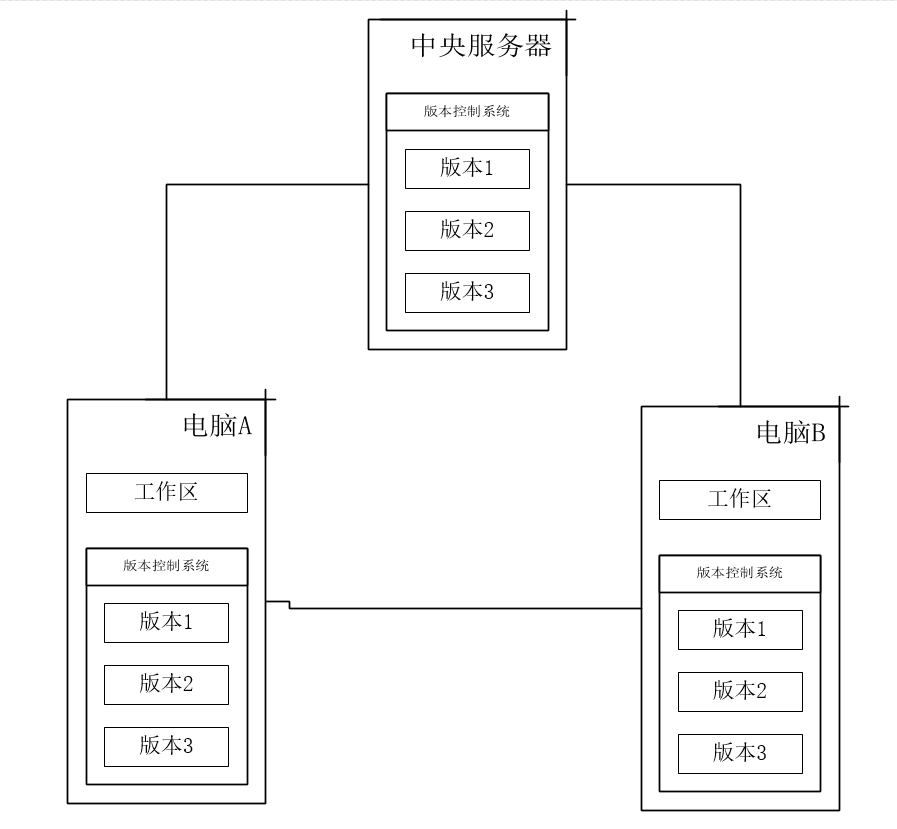
\includegraphics[width=10cm]{image/git/distri.png}
    \caption{分布式版本控制系统}
    \label{dis-con}
\end{figure}

\subsubsection{Git介绍}
Git是一个分布式版本控制系统,保存的是文件的完整快照,而不是差异变化或者文件补丁。

Git每一次提交都是对项目文件的一个完整拷贝,因此你可以完全恢复到以前的任一个提交而不会发生任何区别。这里有一个问题:如果我的项目大小是10M,那Git占用的空间是不是随着提交次数的增加线性增加呢?我提交(commit)了10次,占用空间是不是100M呢?答案是否,如果文件没有变化,Git只会保存指向上一个版本的文件的指针,即对于一个特定版本的文件,Git只会保存一个副本,但可以有多个指向该文件的指针。如图\ref{git-file}右所示。

\begin{remark}
    \textit{Git最适合保存文本文件,如各种语言的源代码,因为Git可以对文本文件进行很好的压缩和差异分析。而针对视频、图片等二进制文件,Git版本管理并不能取得较好的效果(压缩比率低,不能差异分析)。对于二进制文件,Git压缩率非常小,其占用空间随提交次数几乎线性增长。}
\end{remark}

\begin{figure}[ht]
    \centering
    \begin{minipage}[c]{0.45\textwidth}
        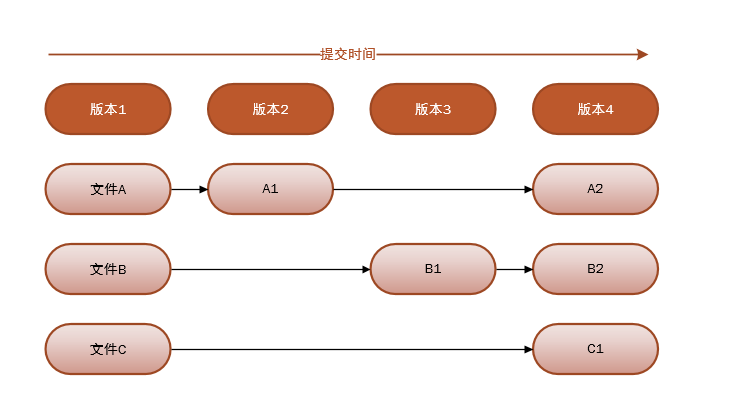
\includegraphics[width=\textwidth]{image/git/git-file.png}
    \end{minipage}
    \begin{minipage}[c]{0.45\textwidth}
        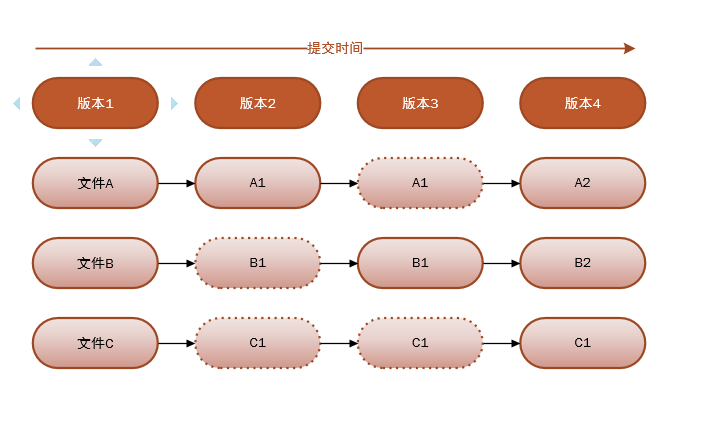
\includegraphics[width=\textwidth]{image/git/git-file2.png}
    \end{minipage}
    \caption{Git的文件管理方式}
    \label{git-file}
\end{figure}

Git有三个工作区域:工作目录,暂存区域,以及本地仓库,三者关系如图\ref{git-workflow}左所示。工作目录是你当前进行工作的区域;暂存区域是你运行git add命令后文件保存的区域,也是下次提交将要保存的文件(注意:Git 提交实际读取的是暂存区域的内容,而与工作区域的文件无关,这也是当你修改了文件之后,如果没有添加git add到暂存区域,并不会保存到版本库的原因);本地仓库就是版本库,记录了你工程某次提交的完整状态和内容,这意味着你的数据永远不会丢失。 file 相应的,文件也有三种状态:已提交(committed),已修改(modified)和已暂存(staged)。已提交表示该文件已经被安全地保存在本地版本库中了;已修改表示修改了某个文件,但还没有提交保存;已暂存表示把已修改的文件放在下次提交时要保存的清单中,即暂存区域。所以使用Git的基本工作流程如图\ref{git-workflow}右所示,即:

\begin{enumerate}
    \item 在工作区域增加,删除或者修改文件。
    \item 用Git将文件快照保存到暂存区域。
    \item 提交更新,将文件永久版保存到版本库中。
\end{enumerate}

\begin{figure}[ht]
    \centering
    \begin{minipage}[c]{0.45\textwidth}
        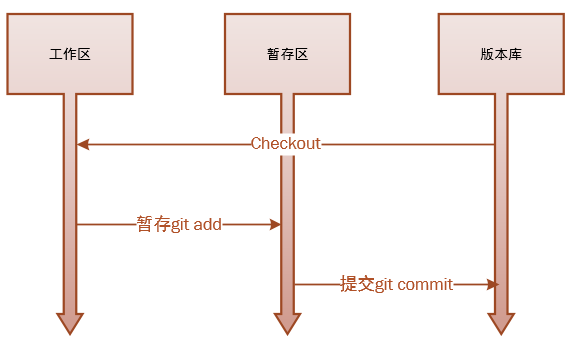
\includegraphics[width=\textwidth]{image/git/git-subarea.png}
    \end{minipage}
    \begin{minipage}[c]{0.45\textwidth}
        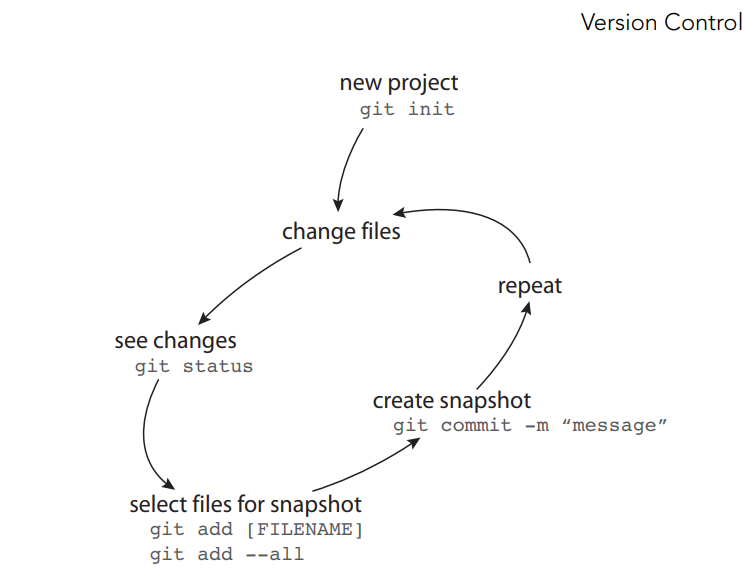
\includegraphics[width=\textwidth]{image/git/git-workflow.PNG}
    \end{minipage}
    \caption{Git分区及各分区关系和使用Git的工作流程}
    \label{git-workflow}
\end{figure}

\subsection{Git的命令操作}
Git 的常用命令分为本地和远程两部分。本地命令主要是在本地进行对代码的版本控制和分支,远程命令则包含了与远程存储库通信的方法。

\subsubsection{Git环境配置}
为了协同和历史查询的方便,Git在操作过程中会记录操作者的有关信息,这些有关信息都可以在.gitconfig文件中进行配置。值得一提的是,为了后续与GitHub传递文件时网络稳定,建议为Git配置代理,Clash for windows默认监听127.0.0.1:7890端口,故配置命令如下:
\begin{lstlisting}
    git config --global user.email "you@example.com"
    git config --global user.name "Your Name"
    git config --global http.proxy http://127.0.0.1:7890
\end{lstlisting}

Windows系统的\lstinline{.gitconfig}文件位于用户文件夹下,是一个隐藏文件,配置完成后\lstinline{.gitconfig}文件内容如下:
\begin{lstlisting}
[user]
	email = 1418767078@qq.com
	name = MingchuanTang
[http]
	proxy = http://127.0.0.1:7890
\end{lstlisting}

\subsubsection{Git本地命令}
\begin{lstlisting}
    ## 版本控制的基本操作
    # 首先需要在工作文件夹下初始化git,生成本地git仓库
    git init
    # 查看git状态:是否有未提交的文件和处在缓存状态下的文件
    git status
    # 提交该文件夹下的所有文件进入缓存状态
    git add .
    # 提交该文件夹下的某个文件
    git add <the file>
    # 将缓存状态下的所有文件提交到本地git仓库
    git commit
    # 输入此次提交的说明信息
    git commit -m "message for the upload"
    # 查看提交的历史记录
    git log
\end{lstlisting}

除此之外,你可以将不需要跟踪/更新的文件加入\lstinline{.gitignore}文件中,这样在git add和git commit操作均不会改变.gitignore中文件的状态。

\subsubsection{Git远程命令}
\label{remote-order}
\begin{lstlisting}
    # 将远程仓库中的内容克隆到本地
    git clone <weblink>
    # 从远程仓库获取更新合并到本地
    git pull
    # 将本地更新提交到远程仓库
    git push
    # 从远程仓库获取更新
    git fetch
    # 查看远程仓库
    git remote
\end{lstlisting}

\subsection{Git的重要功能——分支}
分支(branch)是Git最重要的功能之一\footnote{该部分内容较进阶,在开发新功能、合作完成项目时能起到巨大作用。初学者略读,了解就好,可在实际使用中不断加深对分支的理解。},使用Git可以在工作流程中频繁使用分支与合并,因为Git分支非常轻量级,不像其他的版本控制,创建分支意味着要把项目完整的拷贝一份,而Git创建分支是在瞬间完成的,与工程的复杂程度无关。

与分支有关的操作如下,可通过网站\href{https://learngitbranching.js.org/?locale=zh_CN}{Learn Git Branching}练习分支有关操作。
\begin{lstlisting}
    # 创建分支
    git branch new_branch_name 
    # 转到某个分支,之后的 add ``commit 创建子分支等操作将在此基础上进行
    git checkout exist_branch_name 
    # 创建并转到某个分支
    git checkout -b new_branch_name 
    # 将当前分支和 branch_name 分支合并
    git merge branch_name 
    # 将文件放入暂存区
    git add 
    # 将暂存区内容添加到本地仓库
    git commit 
    # 合并两个分支,最为双方的子节点
    git merge another_branch 
    # 合并分支并将该分支节点作为 another branch 单独的子节点
    git rebase another_branch 
\end{lstlisting}

\subsubsection{分支的创建与切换}
Git的默认分支是master(因为某些原因现在改为了main),存储在\lstinline{.git\refs\heads\master(main)}文件中,假设你在master分支运行\lstinline{git branch dev}创建了一个名字为dev的分支,那么Git所做的实际操作是:

\begin{enumerate}
    \item 在\lstinline{.git\refs\heads}文件夹下新建一个文件名为dev(没有扩展名)的文本文件。
    \item 将HEAD指向的当前分支(当前为master)的40位SHA-1 校验和外加一个换行符写入dev文件。
    \item 结束。
\end{enumerate}

\begin{figure}[ht]
    \centering
    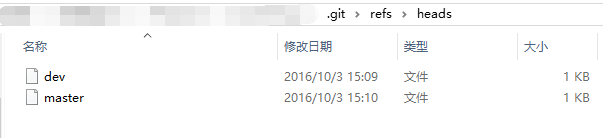
\includegraphics[width=13cm]{image/git/git-branch.png}
    \caption{branch在文件夹中的存储方式}
    \label{git-branch}
\end{figure}

如图\ref{git-branch}所示。

对于切换分支,Git实际完成了如下操作:
\begin{enumerate}
    \item 修改.git文件下的HEAD文件为ref: refs/heads/<分支名称>。
    \item 按照分支指向的提交记录将工作区的文件恢复至一模一样。
    \item 结束。
\end{enumerate}

\subsubsection{分支合并merge}
创建多条分支后,最终都会面临合并到一个主线的问题。合并分支首先是Fast-forward,换句话说,如果顺着一个分支走下去可以到达另一个分支的话,那么 Git 在合并两者时,只会简单地把指针右移,因为这种单线的历史分支不存在任何需要解决的分歧,所以这种合并过程可以称为快进(Fast forward)。如图\ref{merge}上:
\begin{remark}
    \textit{注意箭头方向,因为每一次提交都有一个指向上一次提交的指针,所以箭头方向向左}
\end{remark}

当在master分支合并dev分支时,因为他们在一条线上,这种单线的历史分支不存在任何需要解决的分歧,所以只需要master分支指向dev分支即可,所以很快。

当分支出现分叉时,就有可能出现冲突,而这时Git会要求你去解决冲突,如图\ref{merge}中所示:

因为master分支和dev分支不在一条线上,即v7不是v5的直接祖先,Git 不得不进行一些额外处理。就此例而言,Git 会用两个分支的末端(v7 和 v5)以及它们的共同祖先(v3)进行一次简单的三方合并计算。合并之后会生成一个和并提交v8。

\begin{remark}
    \textit{合并提交有两个祖先(v7和v5)}
\end{remark}

\begin{figure}[ht]
    \centering
    \begin{minipage}[c]{0.9\textwidth}
        \centering
        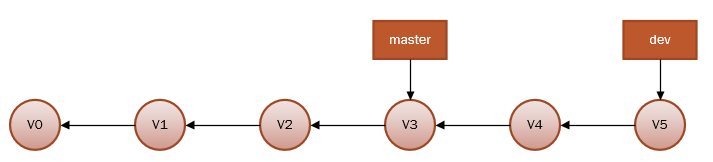
\includegraphics[width=10cm]{image/git/giit-merge.png}
    \end{minipage}

    \begin{minipage}[c]{0.9\textwidth}
        \centering
        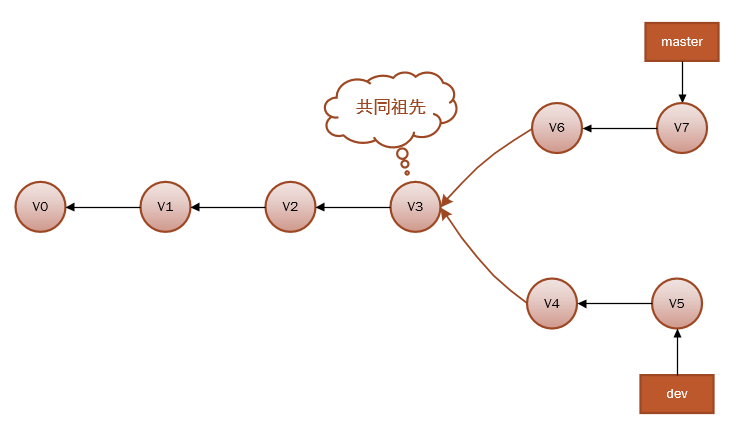
\includegraphics[width=10cm]{image/git/git-merge2.png}
    \end{minipage}

    \begin{minipage}[c]{0.9\textwidth}
        \centering
        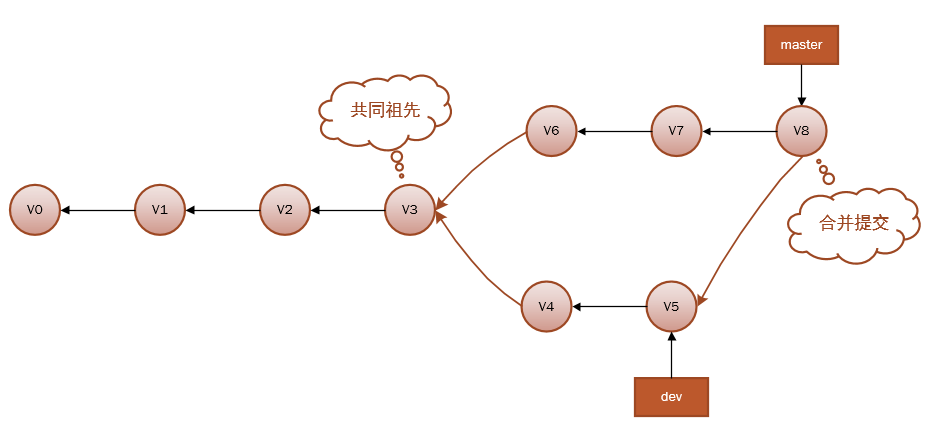
\includegraphics[width=10cm]{image/git/git-merge3.png}
    \end{minipage}
    \caption{Git merge的可能情况}
    \label{merge}
\end{figure}

\subsubsection{分支变基rebase}
把一个分支中的修改整合到另一个分支的办法有两种:merge 和 rebase。merge和rebase最终的结果是一样的,但rebase能产生一个更为整洁的提交历史。仍然以图\ref{rebase}上为例,如果简单的merge,会生成一个提交对象v8,现在我们尝试使用变基合并分支,切换到dev:
\begin{lstlisting}
    git checkout dev
    git rebase master
    # First, rewinding head to replay your work on top of it...
    # Applying: added staged command
\end{lstlisting}

这段代码的意思是:回到两个分支最近的共同祖先v3,根据当前分支(也就是要进行变基的分支 dev)后续的历次提交对象(包括v4,v5),生成一系列文件补丁,然后以基底分支(也就是主干分支 master)最后一个提交对象(v7)为新的出发点,逐个应用之前准备好的补丁文件,最后会生成两个新的合并提交对象(v4',v5'),从而改写 dev 的提交历史,使它成为 master 分支的直接下游,如图\ref{rebase}中:

现在,就可以回到master分支进行快速合并Fast-forward了,因为master分支和dev分支在一条线上,如图\ref{rebase}下:
\begin{lstlisting}
    git checkout master
    git merge dev
\end{lstlisting}

现在的 v5' 对应的快照,其实和普通的三方合并,即上个例子中的 v8 对应的快照内容一模一样。虽然最后整合得到的结果没有任何区别,但变基能产生一个更为整洁的提交历史。如果视察一个变基过的分支的历史记录,看起来会更清楚:仿佛所有修改都是在一根线上先后进行的,尽管实际上它们原本是同时并行发生的。

\begin{figure}[ht]
    \centering
    \begin{minipage}[c]{0.9\textwidth}
        \centering
        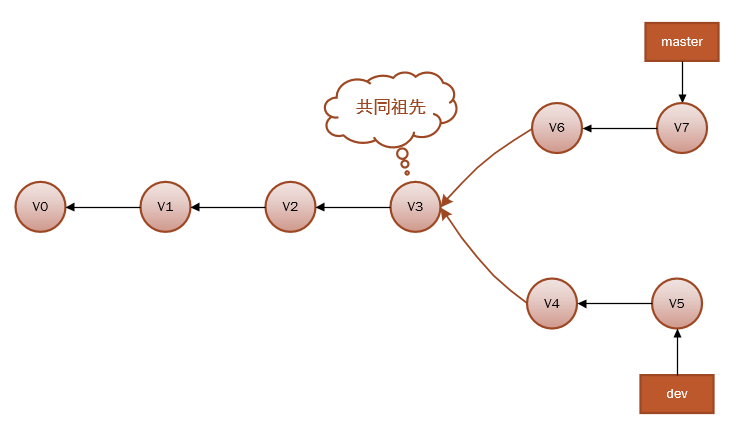
\includegraphics[width=10cm]{image/git/git-rebase.png}
    \end{minipage}

    \begin{minipage}[c]{0.9\textwidth}
        \centering
        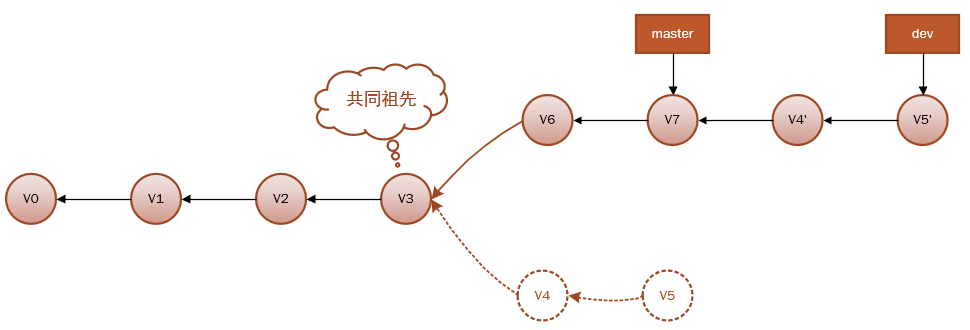
\includegraphics[width=10cm]{image/git/git-rebase2.png}
    \end{minipage}

    \begin{minipage}[c]{0.9\textwidth}
        \centering
        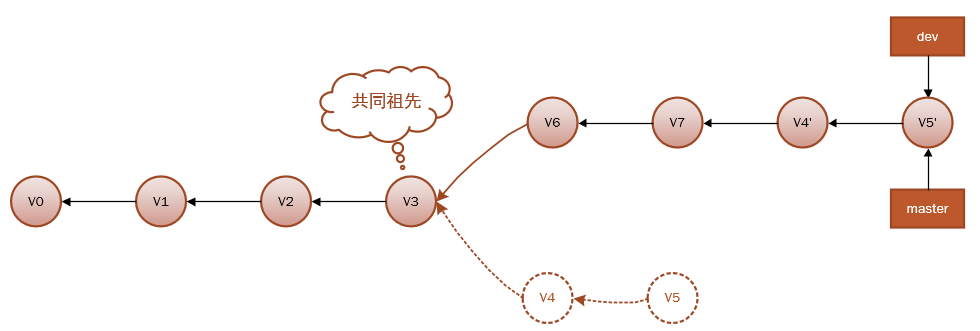
\includegraphics[width=10cm]{image/git/git-rebase3.png}
    \end{minipage}
    \caption{Git rebase过程}
    \label{rebase}
\end{figure}


\section{Github}
GitHub 是一个基于 Git 的远程代码托管仓库,目前由微软公司所有。它提供了一个用户友好的 Web 界面,让开发者可以在浏览器中轻松地管理 Git 仓库。GitHub 不仅提供公共仓库,让开发者可以共享和协作开源项目,还提供私有仓库,供团队内部协作使用。GitHub 的功能包括:代码审查、问题跟踪、团队协作工具、代码托管等。从此前对分布式版本管理系统的描述,你可以看出GitHub的角色就是其中的中央服务器,类似GitHub的平台还有GitLab,Gitolite等。

\begin{remark}
    \textit{Git 和 GitHub 的关系在于,GitHub 是一个基于 Git 的服务。Git 本身是一个独立的分布式版本控制系统,可以在本地和任何远程服务器上使用,而 GitHub 则为 Git 提供了一个便捷的在线平台,使得开发者可以轻松地共享、协作和托管代码。}
\end{remark}

与GitHub相关的Git基本操作见\ref{remote-order},除此之外,为了方便写作GitHub提供了如下功能:
\begin{itemize}
    \item Issue:写出项目的bug等,发起话题供大家讨论
    \item Pull Request \& Merge:远程协作,将自己的代码整合到项目中
    \item Comment:对代码等提出评论
    \item Follow:对项目、开发者、组织等进行关注和跟进
    \item Star:“收藏”功能
\end{itemize}


\subsection{实例:通过GitHub创建小组仓库并同步小组资料}

我们曾在前言中提到小组的GitHub仓库\href{https://github.com/Alchemiiiist/LEB23\_G4}{LEB23\_G4}。该仓库的维护过程正是本节的内容。

\begin{enumerate}
    \item 安装Git
          本部分参考了CSDN上的文章\cite{git-install}。
          通过\href{https://git-scm.com/}{git-scm.com}、\href{https://gitforwindows.org/}{gitforwindows.org}或者\href{https://registry.npmmirror.com/binary.html?path=git-for-windows/}{阿里镜像}下载系统对应的安装包,然后跟随安装指南一步步安装即可。

    \item 配置本地Git(设置用户名和邮箱)
          \begin{lstlisting}
        git config --global user.email "you@example.com"
        git config --global user.name "Your Name"
    \end{lstlisting}

    \item 使用令牌登录

          参考文章:\cite{github-repo}。可在GitHub中获取仓库token(令牌),如图\ref{token}。
          \begin{lstlisting}
        git remote set-url origin https://<your_token>@github.com/<USERNAME>/<REPO>.git
    \end{lstlisting}

          \begin{figure}[ht]
              \begin{minipage}[c]{0.5\textwidth}
                  \centering
                  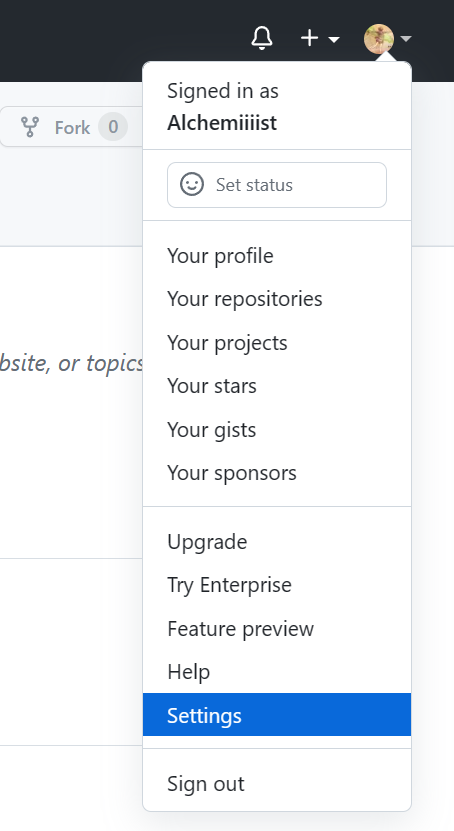
\includegraphics[width=0.5\textwidth]{image/git/github-token.png}
              \end{minipage}
              \begin{minipage}[c]{0.25\textwidth}
                  \centering
                  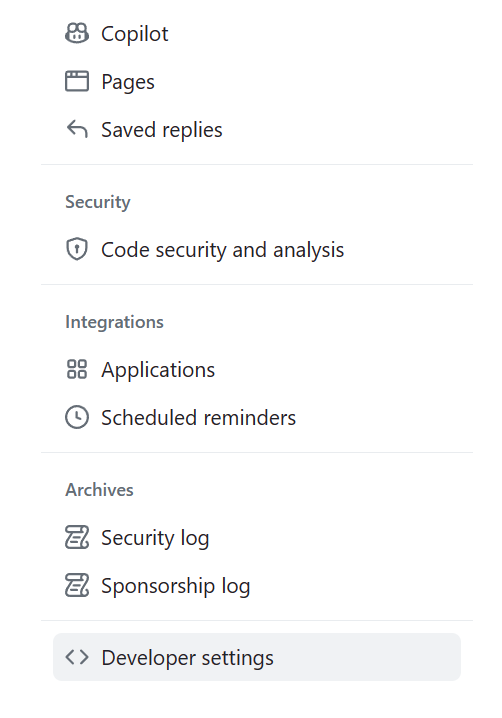
\includegraphics[width=0.5\textwidth]{image/git/github-token2.png}
              \end{minipage}

              \begin{minipage}[c]{0.95\textwidth}
                  \centering
                  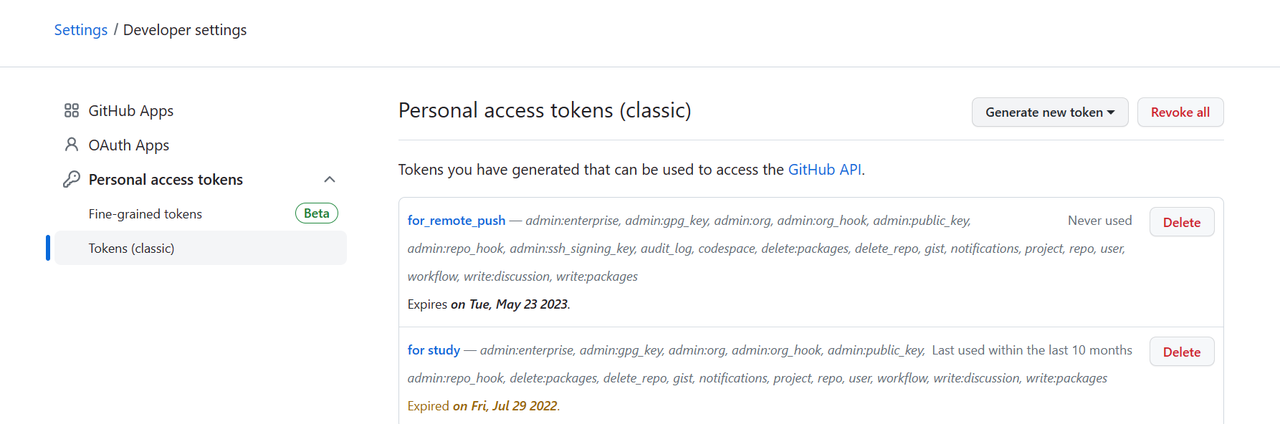
\includegraphics[width=10cm]{image/git/github-token3.png}
              \end{minipage}
              \caption{在GitHub中设置token}
              \label{token}
          \end{figure}

    \item 注册GitHub账号并且建立仓库

          在主页点击-repository-new即可创建仓库,如图\ref{githubrepo}
          \begin{figure}[ht]
              \centering
              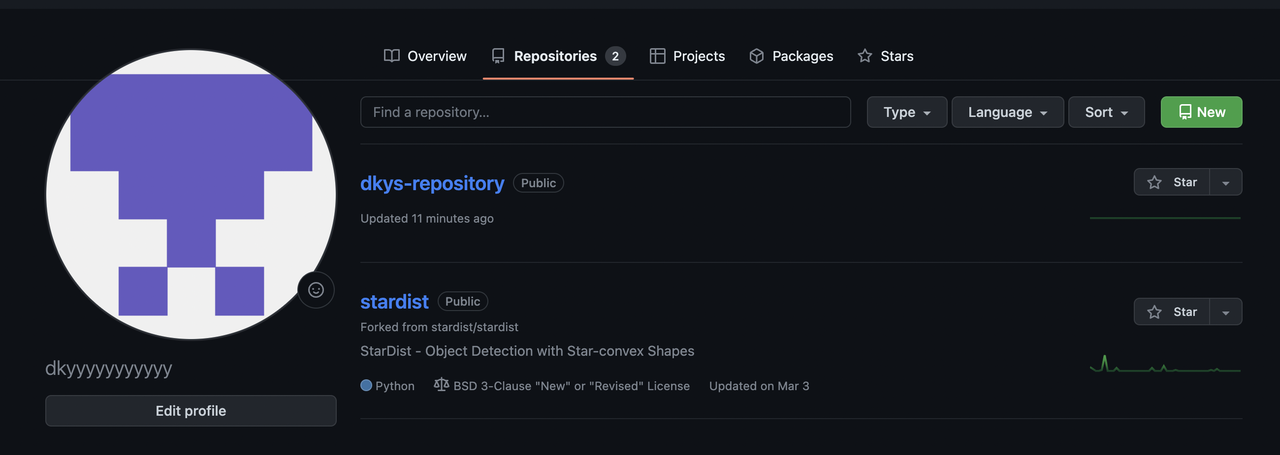
\includegraphics[width=10cm]{image/git/github-repo.png}
              \caption{GitHub仓库}
              \label{githubrepo}
          \end{figure}

          得到仓库地址:https://github.com/dkyyyyyyyyyyy/dkys-repository.git

    \item 本地新建测试文件夹,并且建立与指定远程仓库相同步的本地仓库
          \begin{lstlisting}
        touch 1234.txt
        git clone https://github.com/dkyyyyyyyyyyy/dkys-repository.git
    \end{lstlisting}

    \item 暂存并提交代码
          \begin{lstlisting}
        git add *
        git commit -m 'messages'
        git branch -M main
        git push origin main(本地):main(远程)
    \end{lstlisting}
          VSCode会自动连接到github询问授权信息,点击同意即可。

    \item 传输完成

          如其他人上传到你的仓库,会收到邮件,最后在网页上同意pull request即可,如图\ref{pull-request}。
          \begin{figure}[ht]
              \begin{minipage}[c]{0.9\textwidth}
                  \centering
                  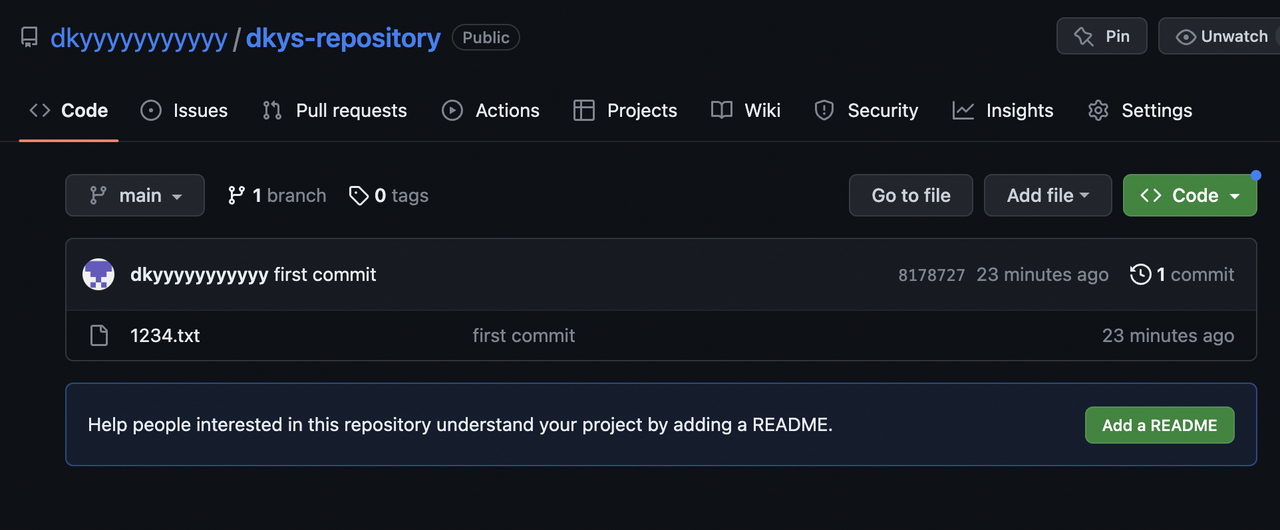
\includegraphics[width=13cm]{image/git/github-upload.png}
              \end{minipage}

              \begin{minipage}[c]{0.25\textwidth}
                  \centering
                  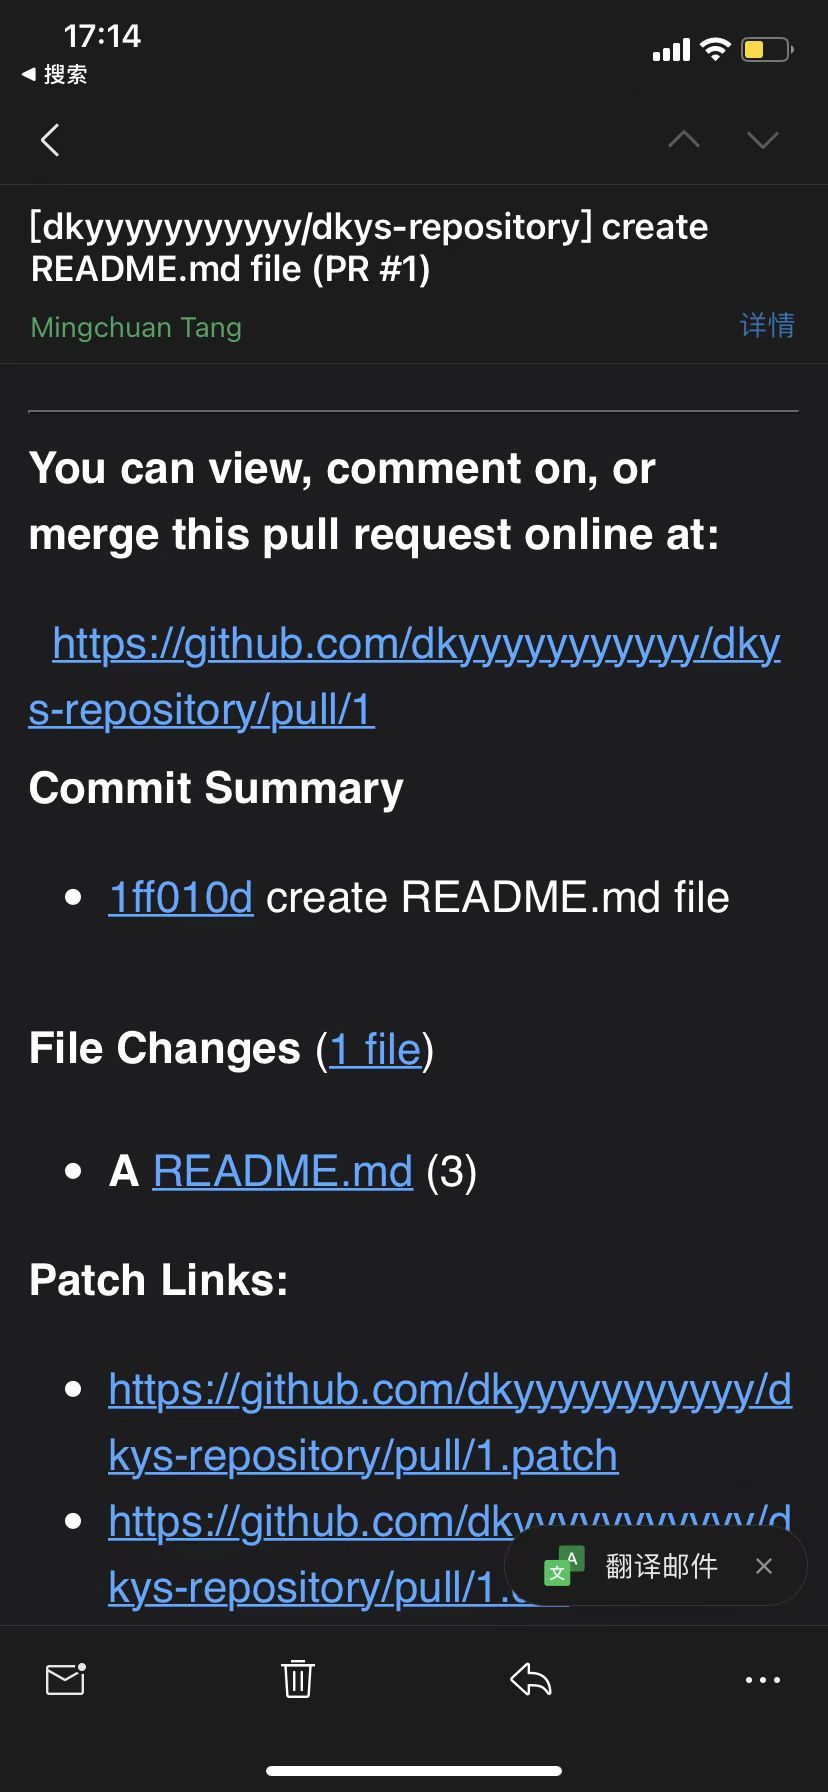
\includegraphics[width=0.9\textwidth]{image/git/github-pullrequest.jpg}
              \end{minipage}
              \begin{minipage}[c]{0.6\textwidth}
                  \centering
                  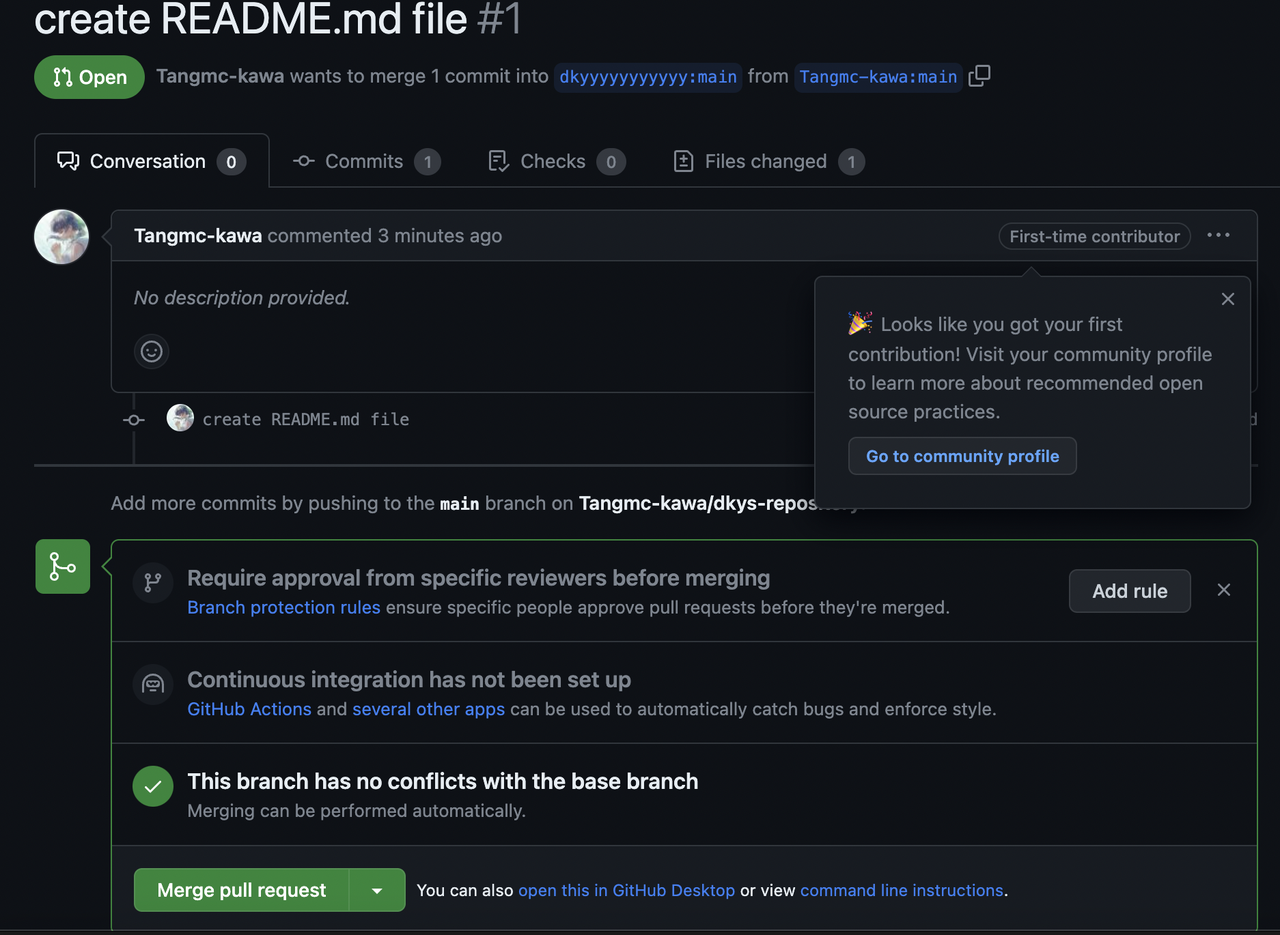
\includegraphics[width=0.9\textwidth]{image/git/github-pullrequest2.jpg}
              \end{minipage}
              \caption{git pull request}
              \label{pull-request}
          \end{figure}

\end{enumerate}

\subsubsection{注意事项}
一般来说,针对自己的GitHub仓库,直接push即可将本地文件与云端同步,但是对于其他人的GitHub仓库,若没有token,则协作的一般过程是在网页端将他人的仓库fork到自己的仓库,然后在本地克隆fork的仓库。本地进行的修改将和自己fork的仓库同步,最后在网页端向原仓库发起pull request(即请求将自己的修改merge到原仓库中),由原仓库端消除冲突后即可完成对原项目的贡献,你的GitHub账户也会出现在原仓库的contributor列表中。

若有token,则可按照上述步骤直接对原仓库进行修改,所以切记,保护好自己的token,不要轻易泄露,以防对自己的项目造成不可估量的损失。


\section{实例:VSCode中利用Git和GitHub管理文件}
VSCode自带Source control功能,可以在此进行commit、push等行为。特别的是,如果需要对其他项目进行协作,vscode能自动完成创建fork(为用户创建一个原文件的复制)和pull and push(将本地和云端仓库同步)的工作,省去很多麻烦。

\begin{figure}[ht]
    \begin{minipage}[c]{0.4\textwidth}
        \centering
        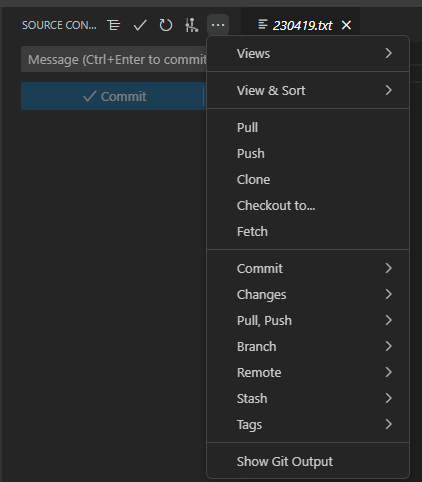
\includegraphics[width=0.95\textwidth]{image/git/github-source-con.png}
    \end{minipage}
    \begin{minipage}[c]{0.35\textwidth}
        \centering
        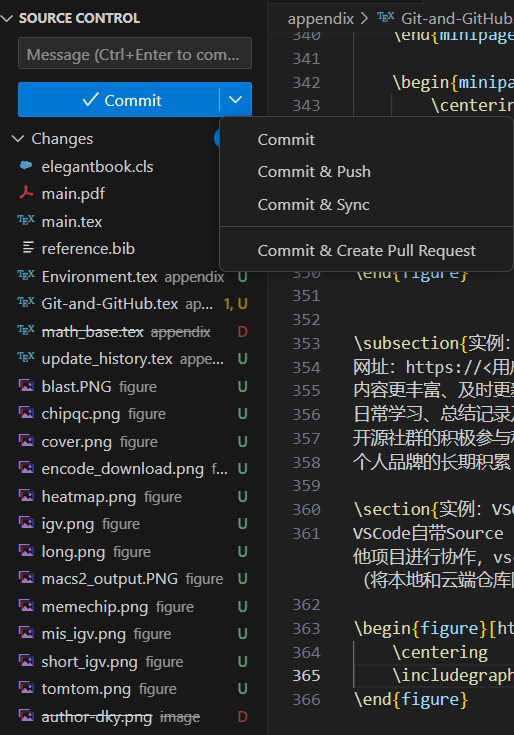
\includegraphics[width=0.95\textwidth]{image/git/github-source-con2.png}
    \end{minipage}
    \begin{minipage}[c]{0.2\textwidth}
        \centering
        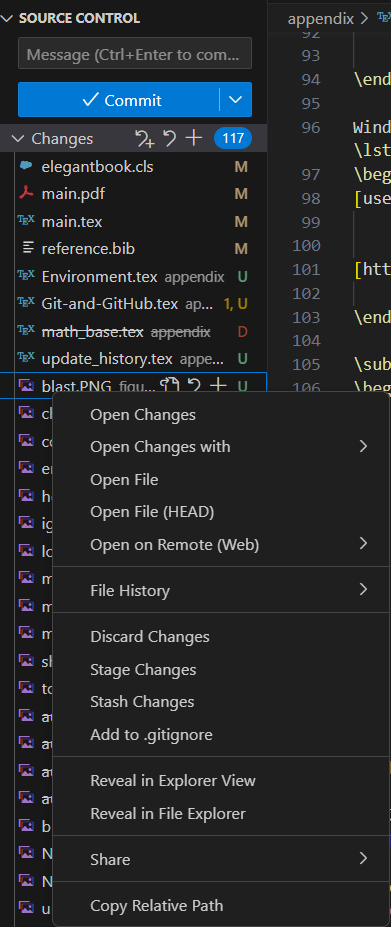
\includegraphics[width=0.95\textwidth]{image/git/github-source-con3.png}
    \end{minipage}
    \caption{VSCode的Source Control功能实现Git所有操作}
    \label{source-con}
\end{figure}

如图\ref{source-con}中所示,如果用GitHub打开一个含.git文件夹的目录(经过git init的目录),则可在Source Control页面查看当前的文件状态,其中M表示修改,U表示新加,D表示删除。同时可右键点击某文件对其进行单独处理,如图\ref{source-con}右所示。